\documentclass{beamer}
\setbeamertemplate{caption}[numbered]{}
\usepackage{multicol}
\usepackage{tikz}
\usepackage{pgfplots}
\usepackage{setspace}
\newcommand{\per}{\mathrm{Per}}
\newcommand{\eat}[1]{}
\newcommand{\topic}[1]{\noindent{{\bf #1}:}}
\newcommand{\calX}{{\mathcal X}}
\newcommand{\calH}{{\mathcal H}}
\newcommand{\calC}{{\mathcal C}}
\newcommand{\calD}{{\mathcal D}}
\newcommand{\calL}{{\mathcal L}}
\newcommand{\calF}{{\mathcal F}}
\newcommand{\calP}{{\mathcal P}}
\newcommand{\calS}{{\mathcal S}}
\newcommand{\calT}{{\mathcal T}}
\newcommand{\calM}{{\mathcal M}}
\newcommand{\calN}{{\mathcal N}}
\newcommand{\calR}{{\mathcal R}}
\newcommand{\tuple}[1]{\left(#1\right)}
\newcommand{\set}[1]{\left\{#1\right\}}
\newcommand{\defeq}{\triangleq}

\newcommand{\Prob}{{\operatorname{Pr}}}
\newcommand{\Exp}{{\mathbb{E}}}
\newcommand{\E}{{\mathbb{E}}}
\newcommand{\G}{{\mathcal{G}}}
\newcommand{\R}{{\mathbf{R}}}
\renewcommand{\H}{{\mathcal{H}}}
\newcommand{\T}{{\mathcal{T}}}
\renewcommand{\P}{{\mathcal P}}
\renewcommand{\r}{{\mathbf{r}}}

\newcommand{\hpf}{\Psi(\calP)}

\newcommand{\Var}{\operatorname{Var}}
\newcommand{\dist}{\mathrm{d}}
\renewcommand{\d}{\mathrm{d}}

\newcommand{\depth}{\mathsf{depth}}
\newcommand{\rank}{\mathsf{rank}}
\newcommand{\opt}{\mathsf{OPT}}
\newcommand{\sol}{\mathsf{SOL}}
\newcommand{\vol}{\mathsf{vol}}
\newcommand{\cost}{\mathsf{cost}}
\newcommand{\FA}{\mathrm{FPRAS}}
\newcommand{\sharpP}{\#\mathrm{P}}
\newcommand{\inapp}{\mathrm{Inapprox}}
\newcommand{\open}{\mathrm{Open}}

\newcommand{\B}{\mathsf{B}}

\newcommand{\tB}{\widetilde{B}}
\newcommand{\A}[1]{\langle #1\rangle}
\newcommand{\e}{\epsilon}
\newcommand{\bS}{\bar{S}}

\newcommand{\true}{\mathsf{true}}
\newcommand{\false}{\mathsf{false}}

\newcommand{\hx}{\widehat{x}}
\newcommand{\hy}{\widehat{y}}
\newcommand{\hz}{\widehat{z}}
\newcommand{\tx}{\widetilde{x}}
\newcommand{\ty}{\widetilde{y}}
\newcommand{\tz}{\widetilde{z}}
\newcommand{\hg}{\widehat{g}}
\newcommand{\bg}{\bar{g}}
\newcommand{\bd}{\bar{d}}
\newcommand{\td}{\tilde{d}}
\newcommand{\V}{\mathcal{V}}
\renewcommand{\L}{\mathsf{T}}
\newcommand{\U}{\mathcal{U}}

\newcommand{\iin}{\mathsf{In}}
\newcommand{\poly}{\mathrm{poly}}

%\newcommand{\diam}{\mathsf{D}}
%\newcommand{\C}{\mathsf{C}}
%\newcommand{\DCP}{\mathsf{DCP}}
%\newcommand{\CP}{\mathsf{CP}}
%\newcommand{\MST}{\mathsf{MST}}
%\newcommand{\M}{\mathsf{M}}
%\newcommand{\MM}{\mathsf{MPM}}
%\newcommand{\CC}{\mathsf{CC}}
%\newcommand{\CH}{\mathsf{CH}}
%\newcommand{\DT}{\mathsf{DT}}
\newcommand{\diam}{\mathrm{diam}}
\newcommand{\D}{\mathsf{D}}
\newcommand{\C}{\mathsf{C}}
\newcommand{\DCP}{\mathsf{C}}
\newcommand{\KCP}{\mathsf{kC}}
\newcommand{\CP}{\mathsf{CP}}
\newcommand{\KC}{\mathsf{kCL}}
\newcommand{\MST}{\mathsf{MST}}
\newcommand{\CH}{\mathsf{C}}
\newcommand{\DT}{\mathsf{C}}
\newcommand{\NN}{\mathsf{NN}}
\newcommand{\KMNN}{\mathsf{kmNN}}

\newcommand{\core}{stoch-core}
\newcommand{\MM}{{\textsf{MAXIMUM-ELEMENT}}}
\newcommand{\mm}{{\textsf{MINIMUM-ELEMENT}}}
\newcommand{\MS}{{\textsf{MAX-SUM}}}
\newcommand{\ms}{{\textsf{MIN-SUM}}}
\newcommand{\ES}{{\textsf{EXACT-SUM}}}
\renewcommand{\d}{\mathrm{d}}
\newcommand{\p}{p}
\newcommand{\Cl}{\mathsf{Cl}}
\newcommand{\Home}{\mathcal{H}}

\newcommand{\etal}{et al. }
\newcommand{\realize}{\vDash}
\newcommand{\consistent}{\thicksim}
\newcommand{\red}[1]{\textcolor{red}{#1}}

\newcommand{\handr}{\textcolor{magenta}{\HandRight}}
\newcommand{\zhuyi}{\noindent\alert{\handr}}
\newtheorem{conjecture}{Conjecture}
\newcommand{\rmnum}[1]{\romannumeral #1}
\newcommand{\Rmnum}[1]{\expandafter\@slowromancap\romannumeral #1@}

\mode<presentation> {
\usetheme{Madrid}
}
\eat{
v\title[Short title]{Stochastic Extreme Value Optimization} 
\author{Liu Yu} 
\institute[IIIS] 
{
Tsinghua University \\ 
\medskip
\textit{liuyujyyz@gmail.com} 
}
\date{\today} 
}
\newif\iflattersubsect
%%%%%%%%%%%%%%%%%%%%%%%%%%%%%%%%%%%%%%%%%%%%%%%%%%%%%%%%%%%%%%%%%%%%%%%%%%%%%%%%%%%%%%%%%%%%%%%%%%%%

\begin{document}
\AtBeginSection[]
{
    \frametitle{}\small
   \begin{frame}
    \frametitle{Overview} %
    \tableofcontents[currentsection]
    \end{frame}
    \lattersubsectfalse
}

\AtBeginSubsection[] {
    \iflattersubsect
    \begin{frame}
    \frametitle{Overview} %
    \tableofcontents[currentsubsection]
    \end{frame}
    \fi
    \lattersubsecttrue
}

\title[Thesis Defence]{Stochastic Extreme Value Optimization}
\author[]{Yu Liu\\Advisor: Jian Li\\[0.5em]Email:~\href{liuyujyyz@gmail.com}{\color{blue!70}\texttt{liuyujyyz@gmail.com}}}
\institute[Tsinghua Unversity]{\textcolor{olive}{Institute of Interdisciplinary Information Sciences \\
Tsinghua University
}}
\date{}
%\titlegraphic{\quad \quad \quad \quad \quad \quad \quad \quad \quad \quad \ \ 
\includegraphics[scale = 0.1]{tsinghua.png}}

\begin{frame}
\titlepage
\end{frame}


\begin{frame}
\frametitle{Overview} 
\tableofcontents 
\end{frame}

\section{Introduction}

\begin{frame}
\frametitle{Interview Scheduling}
Alice is finding a job. Alice makes a simple survey about all companies she is interested. She estimates the salary distributions according to her condition.
\begin{spacing}{2.0}

\end{spacing}
However, Alice has to choose some companies and only attends interviews of these company. Alice will choose an offer with the highest salary.
\begin{spacing}{2.0}

\end{spacing}
Which companies should Alice choose to maximize her expected salary?
%\end{spacing}
\end{frame}

\begin{frame}
\frametitle{Bandit Play}

There are 3 bandits:\\
\begin{center}
\begin{tabular}{|ll|ll|ll|}
\hline
Bandit 1& & Bandit 2& &Bandit 3& \\
\hline
 $0$& $0$ &  $0$& $\frac{1}{2}$ & $0$& $\frac{2}{3}$\\
\hline
 $1$& $1$ &  $2$& $\frac{1}{2}$  & $3$& $\frac{1}{3}$\\
\hline
\end{tabular}
\end{center}

\only<2-4>{
You are charged by 1. You can only play one bandit and take the reward.
\begin{center}
\begin{tabular}{c c c}
\only<3-4>{$\Exp[X_i]$ & &$\Pr[X_i > 1]$\\}
\only<4>{All the same: 1& & Bandit 2: $\frac{1}{2}$}
\end{tabular}
\end{center}
}
\only<5->{
You are charged by 1.5. But you can play two of them and take one reward.
\begin{spacing}{2.0}
\begin{center}
\begin{tabular}{c c c}
    \only<6->{& $\Exp[\max(X_i, X_j)]$ &$\Pr[\max(X_i, X_j) > 1.5]$\\}
    \only<7->{
        Bandit 2, 3: & {\color{red}$\frac{5}{3}$} & {\color{red}$\frac{2}{3}$}\\
        Bandit 1, 3: & {\color{red}$\frac{5}{3}$} & $\frac{1}{3}$\\
        Bandit 1, 2: & $\frac{3}{2}$ & $\frac{1}{2}$\\
    }
\end{tabular}
\end{center}
\end{spacing}
}
\end{frame}

\begin{frame}
\frametitle{Problem Definition}
    \begin{itemize}
    \item Input 1: a set of choices (companies, bandits);
	\item Input 2: a collection of feasible choice sets (time cost, number of plays);
	\item Output: a feasible set, which maximizes the expected value of the best choice.
	\end{itemize}
\begin{problem}[$\MM$]
Input:
\begin{itemize}
\item a set of independent random variables $\{X_i\}$;
\item a collection of feasible set $\calF \subset 2^{[n]}$ (Constraint);
\end{itemize}
Output:
\begin{itemize}
\item a set $S\in \calF$, which maximizes $\Exp[\max_{i\in S} X_i]$.
\end{itemize}
\end{problem}

Minimization version: minimize $\Exp[\max_{i\in S} X_i]$.

\mm: minimize $\Exp[\min_{i\in S} X_i]$.
\end{frame}

\begin{frame}
\frametitle{Examples of Constraints}
\begin{itemize}
\item Cardinality Constraint: $\{S \mid |S| = K\}$;
\item Cost Constraint: $\{S \mid \sum_{i\in S} c_i \leq C\}$;
\item Path Constraint: paths from $s$ to $t$;
\item Cut Constraint: edges between set $V$ and $\bar V$;
\item Matroid Constraint: $([n], \calF)$ consists a Matoid;
\item ...
\end{itemize}
\end{frame}

\begin{frame}
    \frametitle{Adaptivity}
    \begin{itemize}
        \item Adaptive Algorithm: take a choice and observe the reward, make the next decision accoring to the reward.
        \item Non-adaptive Algorithm: make decisions offline, no matter what the reward is.
    \end{itemize}
\end{frame}

\begin{frame}
\frametitle{Related Work}
\begin{itemize}
    \item Goel \etal studied a variant of knapsack problem and obtain a $\frac{1}{4}(1 - \frac{1}{e})$-approximation algorithm for \MM\ under Cost Constraint.\cite{Goel:asking}
    \item Guha \etal studied the Lagrangian version with Cost Constraint, and proved it can be solved optimally.\cite{Guha07informationacquisition}
    \item Chen \etal studied an online problem and proposed a $1-\frac{1}{e}$-approximation offline algorithm for \MM under Cardinality Constraint.\cite{NIPS2016:MAB}
    \item Goel \etal studied \mm\ deeply and obtained some important results:\cite{Goel:probe}
    \begin{itemize}
        \item Proved it is NP-hard to approximate with any polynomial ratio under the Cost Constraint.
        \item Proposed the CIP (Covering Integer Program) approach to design bi-criteria $(1+\varepsilon)$-approximation algorithm with extra cost.
    \end{itemize}
\end{itemize}
\end{frame}

\begin{frame}
    \frametitle{Notations}
    \begin{itemize}
        \item A discrete random variable $X_i$ takes value over the support set$\{a_{i,1}, \ldots, a_{i, s_i}\}$, with probability $\Pr[X_i = a_{i,j}] = p_{i,j}$. In problems, it is inputed using $\{a_{i,j}\}$ and $\{p_{i,j}\}$.
        \item A Bernoulli random variable has support set with only one non-zero value.
        \item A constraint $\calF$ can have exponential size. Assume it can be represented implictly, i.e., matroid, paths, cuts, forests, ...
    \end{itemize}
\end{frame}

\section{MAXIMUM-ELEMENT}

\begin{frame}
\frametitle{Our Contributions}
\begin{itemize}
    \item In previous work, people design approximation algorithms based on $\Exp[\max_{i\in S} X_i]$ is submodular; In our work, we introduced the truncation trick used in similar problems~\cite{kleinberg2000allocating,guha2009exceeding}. Our algorithm works under more kinds of constraints.
    \item We first propose a PTAS for \MM\ using the discretization and enumeration technique.
\end{itemize}
\end{frame}


\begin{frame}
    \frametitle{Related Problems}
    \begin{problem}[MAX-SUM]
        Input: Given a set of numbers $\{v_i\}$ and a constraint $\calF$;\\
        Output: a set $S\in \calF$ maximizing $\sum_{i\in S} v_i$.
    \end{problem}
    \begin{problem}[MIN-SUM]
        Input: Given a set of numbers $\{v_i\}$ and a constraint $\calF$;\\
        Output: a set $S\in\calF$ minimizing $\sum_{i\in S} v_i$.
    \end{problem}
    \begin{problem}[EXACT-SUM]
        Input: Given a set of integers $\{v_i\}$, a target $T$ and a constraint $\calF$;\\
        Output: a set $S\in \calF$ with $\sum_{i\in S} v_i = T$.
    \end{problem}
\end{frame}

\begin{frame}
\frametitle{Results}
\begin{theorem}[Main Theorem]
    \begin{enumerate}
        \item    There is a constant approximation algorithm for \MM, if there is a constant approximation algorithm for \MS;
        \item    There is a constant approximation algorithm for minimization version \MM, if there is a constant approximation algorithm for \ms;
        \item    There are PTAS for both \MM\ and minimization version of \MM, if there is a psuedo-polynomial time algorithm for \ES.
\end{enumerate}
\end{theorem}
\end{frame}

\begin{frame}
    \frametitle{Constant Approximation}

    \begin{lemma}
        For any set $S$ and constant $T$, if $\Exp[\sum_{i\in S} \max(X_i - T, 0)] \geq T$, we have
        $$\Exp[\max_{i\in S} X_i] \geq T.$$
    \end{lemma}

    Find a $T$ such that:
    \begin{itemize}
        \item For all set $S\in \calF$, $\Exp[\sum_{i\in S} \max(X_i - T, 0)] < T$ (provide a upper bound for optimal solution);
        \item Exist a set $\sol$, $\Exp[\sum_{i\in \sol} \max(X_i - T, 0)] \geq T$ (provide a lower bound for algorithm output).
    \end{itemize}
\end{frame}

\begin{frame}
    \frametitle{Bernoulli Decomposition}
    \begin{definition}[Bernoulli Decomposition]
        Given a discrete random variable $X$, its Bernoulli decomposition is a set of Bernoulli random variables $\{Z_j\}$ such that $X\sim \max_j Z_j$.
    \end{definition}
    If $\Pr[X = a_j] = p_j$, for $j = 1, \ldots, N$, 
    $$Z_j = \left\{
        \begin{array}{ll}
            a_j & \text{with probability} \frac{\Pr[X = a_j]}{\Pr[X \leq a_j]},\\
            0 & \text{otherwise}.
        \end{array}
        \right.
        $$
\end{frame}

\begin{frame}
    \frametitle{PTAS: Discretization}
    \begin{itemize}
        \item    We first run a constant approximation algorithm to obtain an approximation solution $S$.\\
        \item    We discretize input distributions using their Bernoulli decomposition according to the value $M = \Exp[\max_{i\in S} X_i]$.\\
        \item    After discretization step we get:
    \begin{itemize}
        \item A set $\mathsf{Supp}$ of size $O(\frac{1}{\varepsilon^2})$;
        \item $n$ random variables $\bar X_1, \ldots, \bar X_n$ taking values over set $\mathsf{Supp}$.
        \item The optimal solution for $\{\bar X_i\}$ is close to the one for $\{X_i\}$.
    \end{itemize}
    \end{itemize}

\end{frame}
\begin{frame}
    \frametitle{Discretization}
    \begin{figure}
    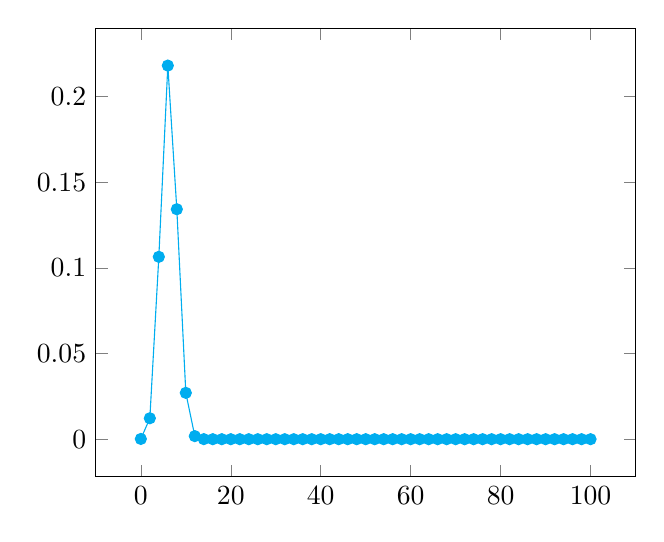
\begin{tikzpicture}[
    declare function={binomcoeff(\n,\k)=\n!/(\k!*(\n-\k)!);},
    declare function={
        hypergeompmf(\N,\K,\n,\k)=binomcoeff(\K,\k)*binomcoeff(\N-\K, \n-\k)/binomcoeff(\N,\n);}
    ]
    \begin{axis}[
        samples at={0,2,...,98,100},
        %ycomb,
        yticklabel style={
            /pgf/number format/fixed,
   %         /pgf/number format/fixed zerofill,
     %       /pgf/number format/precision=1
        },
%        every axis legend/.append style={at={(0.2,0.6)}, anchor=south}
    ]
    \addplot [mark=*, cyan] {hypergeompmf(80,25,20,x)};
    \end{axis}
    \end{tikzpicture}
    \caption{A distribution with many supports and long tail.}
\end{figure}
\end{frame}

\begin{frame}
    \frametitle{Discretization}
    \begin{multicols}{2}
    \begin{figure}
    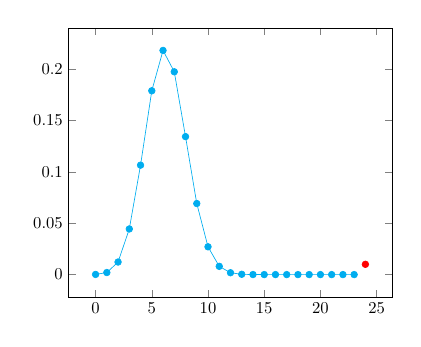
\begin{tikzpicture}[
            scale = 0.6,
    declare function={binomcoeff(\n,\k)=\n!/(\k!*(\n-\k)!);},
    declare function={
        hypergeompmf(\N,\K,\n,\k)=binomcoeff(\K,\k)*binomcoeff(\N-\K, \n-\k)/binomcoeff(\N,\n);}
    ]
    \begin{axis}[
        samples at={0,1,...,22,23},
        yticklabel style={
             /pgf/number format/fixed,
       %     /pgf/number format/fixed zerofill,
        %    /pgf/number format/precision=1
         },
%        every axis legend/.append style={at={(0.2,0.6)}, anchor=south}
    ]
    \addplot [mark=*, cyan] {hypergeompmf(80,25,20,x)};
    \addplot [mark=*, red] coordinates {(24, {0.01})};
    \end{axis}
    \end{tikzpicture}
    \caption{Cut the tail of the distribution.}
    \end{figure}%
%\end{frame}
%\begin{frame}
    \begin{figure}
    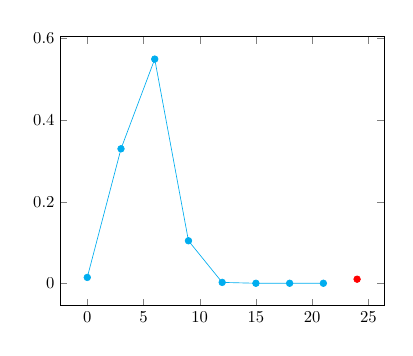
\begin{tikzpicture}[
            scale = 0.6,
    declare function={binomcoeff(\n,\k)=\n!/(\k!*(\n-\k)!);},
    declare function={
        hypergeommf(\N,\K,\n,\k)=binomcoeff(\K,\k)*binomcoeff(\N-\K, \n-\k)/binomcoeff(\N,\n);},
    declare function={
        hyperadd(\N,\K,\n,\k)=hypergeommf(\N,\K,\n,\k)+hypergeommf(\N,\K,\n,\k+1)+hypergeommf(\N,\K,\n,\k+2);}
    ]
    \begin{axis}[
        samples at={0,3,...,21},
        %ycomb,
        %yticklabel style={
        %    /pgf/number format/fixed,
            %/pgf/number format/fixed zerofill,
            %/pgf/number format/precision=1
        %},
%        every axis legend/.append style={at={(0.2,0.6)}, anchor=south}
    ]
    \addplot [mark=*, cyan] {hyperadd(80,25,20,x)};
    \addplot [mark=*, red] coordinates {(24, {0.01})};
    \end{axis}
    \end{tikzpicture}
    \caption{Discretize supports with small steps.}
    \end{figure}
\end{multicols}
\end{frame}

\begin{frame}
    \frametitle{PTAS: Signatures}
    \begin{itemize}
        \item Inputs: $\{\bar X_i\}$ on $\mathsf{Supp}$. $\bar X_i$ can be Bernoulli decomposed to $\{Y_{i,j}\}_{j=1}^z$.
        \item Define Signature for $\bar X_i$ using $\log\Pr[Y_{i,j} = 0]$:
            $$\mathsf{Sig}(\bar X_i) = (\lfloor \frac{-\log(q_{i,1})}{\varepsilon^4 / n}\rfloor\varepsilon^4/n, \cdots, \lfloor \frac{-\log(q_{i,z})}{\varepsilon^4 / n}\rfloor\varepsilon^4/n)$$
            \begin{block}{Fact}
                \begin{itemize}
                    \item $\Exp[\max_{i\in S} \bar X_i]$ takes value on $\mathsf{Supp}$, and can be Bernoulli decomposed to $\{BD_{S,j}\}_{j=1}^z$.\\ 
                    \item $BD_{S,j} = \max_{i\in S} Y_{i,j}$, and $\Pr[BD_{S,j} = 0] = \prod_{i\in S} \Pr[Y_{i,j} = 0]$.
                \end{itemize}
            \end{block}
        \item Define Signature for set $S$ as $$\mathsf{Sig}(S) = \sum_{i\in S} \mathsf{Sig}(\bar X_i).$$ 
    \end{itemize}
\end{frame}

\begin{frame}
    \frametitle{Signatures}
    \begin{lemma}
        If two sets have the same signature, their objective values differ at most $O(\varepsilon) W$.
    \end{lemma}
    \begin{spacing}{2.0}
    \onslide<2->{
        For two sets $S_1$ and $S_2$, $\mathsf{Sig}(S_1) = \mathsf{Sig}(S_2).$\\}
    \onslide<3->{$\Rightarrow$ $\sum_{S_1} \mathsf{Sig}(X_i) = \sum_{S_2} \mathsf{Sig}(X_i)$.\\}
    \onslide<4->{$\Rightarrow$ {\color{red}$\sum_{S_1} \log(q_{i,j})$} is close to {\color{red} $\sum_{S_2} \log(q_{i,j})$} for any $j$.\\}
    \onslide<5->{$\Rightarrow$ {\color{red}$\prod_{S_1} q_{i,j}$} is close to {\color{red}$\prod_{S_2}q_{i,j}$} for any $j$.\\}
    \onslide<6->{$\Rightarrow$ {\color{red}$BD_{S_1,j}$} is close to {\color{red}$BD_{S_2, j}$} for any $j$.\\}
    \onslide<7->{$\Rightarrow$ {\color{red}$\Exp[\max_{S_1} \bar X_i]$} is close to {\color{red}$\Exp[\max_{S_2} \bar X_i]$}.\\}
\end{spacing}
\end{frame}

\begin{frame}
    \frametitle{PTAS: Enumeration}
    \begin{enumerate}
        \item Enumerate possible signatures of sets.
        \item For each signature, try to find a candidate with such signature.\\
            (Quote: Encode signatures to integers and reduce finding a corresponding solution to \ES.)
        \item Return a candidate with the best objective value as solution.
    \end{enumerate}
\end{frame}

\section{MINIMUM-ELEMENT}
\begin{frame}
\frametitle{Our Contributions}
\begin{theorem}
\end{theorem}
\end{frame}

\begin{frame}\frametitle{Thank you!}
Questions?
\end{frame}

\begin{frame}\frametitle{Reference}
\bibliographystyle{plain}
\bibliography{proposal}
\end{frame}
%%%%%%%%%%%%%%%%%%%%%%%%%%%%%%%%%%%%%%%%%%%%%%%%%%%%%%%%%%%%%%%%%%%%%%%%%%%%%%%%%%%%%%%%%%%%%%%%%%%%%%%%%
\end{document}
